\documentclass[12pt]{article}

\usepackage{stylefile}


%% extra layout for QJEP

% double spacing
\usepackage{setspace}
\linespread{1.5}

% larger margins (minimally 1 inch on all sides)
\usepackage[margin = 1.4in]{geometry}

% endnotes (why??)
\usepackage{endnotes}
\let\footnote=\endnote

\begin{document}

\Exlabelsep = 0.2\parindent
\SubExleftmargin = 1.2\parindent

\thispagestyle{empty}


\noindent \LARGE \textbf{Exclusive disjunction}\normalsize \\ [.5cm]
\noindent \large Michael Franke \\ %\vspace{-0.25cm}
\noindent \normalsize Department of Linguistics, University of T\"{u}bingen, Germany \\[.5cm] 
\noindent \large Bob van Tiel\\ %\vspace{-0.25cm}
\noindent \normalsize Department of Languages and Literature, Universit\'{e} Libre de Bruxelles, Belgium


\vspace*{3cm}

\noindent \textbf{Corresponding author:}\\
Michael Franke\\
Department of Linguistics \\
Wilhelmstra\ss e 19\\
72074 T\"{u}bingen\\
Germany\\
\texttt{mchfranke@gmail.com}\\
Tel: +49-7071-2973970\\
Fax: +49-7071-295212

\vspace*{1cm}

\noindent \textbf{Acknowledgements:}\\
MF's work was supported by by the Institutional Strategy of the University of T\"{u}bingen
(Deutsche Forschungsgemeinschaft, ZUK 63) and the Priority Program XPrag.de (DFG
Schwerpunktprogramm 1727). BT's work was supported by the F.R.S.-FNRS Research Incentive Grant F.4502.15 (principal investigator: Mikhail Kissine).

\newpage

\begin{center}
\noindent\LARGE \textbf{Exclusive disjunction}\normalsize\footnote{Word count (including appendices and references): ca.~12,500} \\[.5cm]
% \large Michael Franke\\[.1cm] 
% \large Bob van Tiel
\end{center}

\begin{abstract}
  If someone says ``Donald ate a pretzel or a donut'' the hearer may infer that Donald did not
  eat both a pretzel and a donut. This exclusive reading of ``or'' is often explained as a
  scalar implicature by comparison to an alternative utterance with ``and''. We tested this
  explanation by investigating how the robustness of the exclusive reading of ``or'' is
  influenced by three contextual factors: relevance, competence, and prior probability. We
  found that only prior probability has a significant effect on the robustness of the exclusive
  reading, thus disconfirming the scalar implicature account. Instead, we propose that the
  exclusive reading of ``or'' is a probabilistic inference based on world knowledge.

  \textbf{Keywords:} exclusive disjunction, conversational implicature, pragmatic reasoning, world knowledge
\end{abstract}

%--------------------------------------------------------
\section{Introduction}
%--------------------------------------------------------

Introductions to logic usually distinguish between two readings of ``or'': an inclusive and an exclusive reading \citep[e.g.,][]{mccawley1981, copi2005}. The inclusive reading corresponds to the meaning of logical disjunction. According to this reading, ``$A$ or $B$'' is true if at least one and possibly both of $A$ and $B$ are true. The exclusive reading is more strict in that it excludes the possibility that both $A$ and $B$ are true. So on its exclusive reading, ``$A$ or $B$'' is true if exactly one of $A$ and $B$ is true. To illustrate, consider:

\ex.	\label{ex:support} Joe supports Donald or Hillary.

On its inclusive reading, this sentence is true whenever Joe supports Donald, Hillary, or both. The exclusive reading, which is arguably more prominent in this example, excludes the latter possibility. That is, on its exclusive reading, \Last is true whenever Joe supports Donald or Hillary, but not both.

The presence of these two readings might suggest that ``or'' is associated with two different lexical entries \citep[e.g.,][]{basson1960, baum1996, rescher1964}. There are, however, good reasons to reject such a lexicalist approach. Perhaps the most compelling reason is that, in some contexts, ``or'' can only receive one interpretation. To illustrate, consider the following sentence, in which ``or'' occurs in the scope of negation:

\ex.	 Joe does not support Donald or Hillary.

This sentence has only one interpretation, namely that Joe supports neither Donald nor Hillary \citep[cf.][]{crain2008}. This interpretation corresponds to the inclusive reading of ``or''. It does not have an interpretation corresponding to the exclusive reading; in other words, it does not have a reading according to which Joe either supports both Donald and Hillary, or neither of them. Since ``or'' is systematically monosemous in certain contexts---negation being one of them---it follows that the two readings of ``or'' cannot simply be due to a lexical ambiguity.

An attractive alternative to the lexicalist approach stems from Grice's \citeyearpar{grice1975} theory of conversational implicature. According to Grice, natural conversation is governed by the assumption that speakers are cooperative; that is, they attempt to further the purpose of the discourse by means of their utterances. Speakers are cooperative by adhering to four maxims that enjoin their utterances to be truthful, informative, relevant, and clear. Sometimes hearers have to make ancillary assumptions in order to align a speaker's utterance with the assumption of cooperativity. Such ancillary assumptions are called \emph{conversational implicatures}. An example, from Grice's own work, is given in the following conversation:

\ex.	A: I am out of petrol. \\
 B: There is a garage around the corner.
	
B's utterance would be irrelevant, and hence uncooperative, if he knew that the garage was closed or did not sell petrol. Since A assumes that her interlocutor is cooperative, she thus derives the conversational implicature that the garage is open and sells petrol.

\citet{horn1972} was the first to argue that the exclusive reading of ``or'' can be explained as
a conversational implicature, too, based on the assumption that the primary meaning of ``or'' is
inclusive. To illustrate, consider \ref{ex:support} again. Assuming that the primary meaning of
``or'' is inclusive, the speaker of \ref{ex:support} could have been more informative, and hence
cooperative, by uttering the ``and''-alternative ``Joe supports Donald and Hillary.'' Why didn't
she? Presumably because she does not believe that the ``and''-alternative is true. This is a weak
inference that is compatible with a situation in which the speaker is unsure about whether or
not Joe supports both Donald and Hillary. This weak inference can be strengthened if there is
reason to believe that the speaker knows whether or not Joe supports both Donald and
Hillary. This assumption is often called the \emph{competence assumption}
\citep[e.g.,][]{geurts2010, Russell2006:Against-Grammat, vanRooijSchulz:ExhaustiveInterpretation, ZimmermannFreeChoiceDisjunction2000}. If
the competence assumption is sufficiently plausible, it follows that, according to the speaker,
Joe does not support both Donald and Hillary.

This specific kind of conversational implicature is often called a \emph{scalar implicature} because it is assumed that ``or'' forms a lexical scale with ``and'', and that alternatives are generated by substituting the scalemates ``or'' and ``and''. Other lexical scales are $\langle$some, all$\rangle$, $\langle$warm, hot$\rangle$, and $\langle$intelligent, brilliant$\rangle$.

The implicature account straightforwardly explains the absence of exclusive readings under
negation. Consider \LLast again. Here, unlike in the case of \ref{ex:support}, the
``and''-alternative is less informative than the utterance itself. After all, \LLast is only
compatible with a situation in which Joe supports neither Donald nor Hillary, whereas the
``and''-alternative is also consistent with situations in which Joe supports exactly one of
Donald and Hillary. So the speaker was already maximally informative and hence no implicature
is derived.

Although the implicature account has since become the standard in the literature
\citep[e.g.,][]{chevallier2008, chierchia2012, geurts2010, sauerland2004}, it is not
without its problems, as we will see in the next section. Therefore, we set out to
experimentally test the adequacy of the implicature account. To that end, we investigated the
effect of three factors on the robustness of exclusive readings:\ (i) the \emph{relevance} of
the ``and''-alternative to the hearer, (ii) the \emph{competence} of the speaker about the truth
of the ``and''-alternative, and (iii) the \emph{prior probability} that the ``and''-alternative is
true. These factors are usually taken to influence the robustness of scalar
implicatures. Hence, if the implicature account is correct, we expect these factors to
influence the robustness of the exclusive reading of ``or'', too.

For comparison, we also investigated how relevance, competence, and prior probability influence the robustness of a bona fide scalar implicature, namely the inference from ``some'' to ``not all''. To illustrate, consider:

\ex.	Some of my friends support Donald.

An utterance of this sentence may convey that not all of the speaker's friends support
Donald. The derivation of this upper-bounded construal runs analogous to that of the exclusive
reading of ``or'': the speaker could have been more informative by saying ``All of my friends
support Donald''. Why didn't she? Presumably because she does not believe that this alternative
is true. If, moreover, the speaker knows whether or not all of her friends support Donald---i.e., if the speaker is competent in the relevant sense---it
follows that she believes that not all of her friends support Donald.

As we will see, it turns out that there are marked differences in how relevance, competence, and prior probability influence the robustness of the exclusive reading of ``or'' compared to how they influence the robustness of the inference from ``some'' to ``not all''. These findings will encourage us to reconsider the implicature account of the exclusive reading of ``or''.

In the next section, we explain our three factors of interest in more detail. Afterwards, we outline the details of our experiments and discuss the results.

%--------------------------------------------------------
\section{Relevance, competence, and prior probability}
%--------------------------------------------------------
%--------------------------------------------------------
\subsection*{Relevance}
%--------------------------------------------------------

Almost all theorists agree that the robustness of scalar implicatures is modulated by various extralinguistic factors (e.g., \citealt{chierchia2012, franke2009, geurts2010, horn1972}, but see \citealt{chierchia2004, levinson2000, storto2005}). Some of these factors are specific to certain theories, while others are shared across competing theories. Relevance is of the latter kind in that it features in almost all theories of scalar inferences. However, relevance is a multivocal notion, and there are at least two construals that should be distinguished:\ relevance for the discourse purpose and relevance for the hearer's interest \citep{geurts2010}.

The notion of relevance for the discourse purpose can be illustrated with the following example (from \citealt{kuppevelt1996}):

\ex.	A: How many of the boys were at the party? \\ B: Some of the boys were at the party.

Discourse purposes are usually equated to questions, which can be implicit or, as in this case, explicit \citep{roberts2012}. A piece of information is relevant if it contributes to answering this question. In \Last, the information that not all of the boys went to the party is relevant to the discourse purpose because it narrows down the space of possible answers. Hence, it is hypothesised that ``some'' will be interpreted as ``some but not all''. 

Compare this to a situation in which B's answer addresses the question ``Were some of the boys at the party?'' In this situation, the upper-bounded construal is irrelevant, since the question is already resolved when ``some'' is interpreted as ``at least some and possibly all''. In this situation, then, it is predicted that no scalar implicature will be derived.

In this paper, however, we will mainly be concerned with the second notion of relevance:\ relevance to the hearer's interest. This construal is intimately connected to \emph{relevance theory} \citep{sperber1995}.

According to relevance theory, the relevance of an inference is determined by two factors: (i) the positive cognitive effects it has on the hearer---i.e., to what extent it makes ``a worthwhile difference to the individual's representation of the world'' \citep[p.\ 251]{wilson2002}---and (ii) the effort needed to process that inference. In what follows, we focus on the first factor, assuming that processing effort remains invariant across the scenarios that we tested (cf.\ \citealt{chevallier2008} for a series of experiments on ``or'' that manipulate processing effort). 

The central tenet of relevance theory is that communication is aimed at maximising relevance, so that hearers only derive inferences whose positive cognitive effects outweigh their processing cost. Hence, relevance theory predicts that the robustness of a scalar implicature is an increasing function of its importance to the hearer. To illustrate, consider:

\ex.	Donald won the primaries in Nebraska or Indiana.

According to relevance theory, the robustness of the exclusive reading of this sentence depends on how important it is to the hearer whether Donald won the primaries in both Nebraska and Indiana. Suppose, for example, that the hearer made a large bet that Donald would not win both primaries. In that case, she would be more likely to arrive at an exclusive reading than if, for example, she made a large bet that Donald would win at least one of the primaries.

Hence, if relevance theory is correct, we expect the robustness of the inference from ``some'' to ``not all'' to be positively affected by the relevance of the upper-bounded reading to the hearer. If, in addition, the implicature account is correct, we expect the same effect on the exclusive reading of ``or''.

%--------------------------------------------------------
\subsection*{Competence}
%--------------------------------------------------------

In the previous section, we have seen that competence plays an important role in the derivation of scalar implicatures. Initially, pragmatic reasoning yields a weak inference according to which the speaker does not believe that the more informative alternative is true. This weak inference can be strengthened if the competence assumption holds; that is, if it is assumed that the speaker knows whether or not the more informative statement is true. If so, it follows that, according to the speaker, the more informative statement is false.

Although the workings of the competence assumption tend to be unproblematic for most scalar expressions, they are rather precarious in the case of ``or''. Indeed, the need to invoke competence to arrive at an exclusive reading of ``or'' gives rise to what \citet{zondervan2010} calls the \emph{speaker expertise paradox} \citep[cf.][]{geurts2006}. To explain this paradox, consider \ref{ex:support} once again:

\ex.	Joe supports Donald or Hillary.

We have already seen that someone who utters this sentence is likely to convey that Joe does not support
both Donald and Hillary. Presumably, however, the utterance is also likely to convey that the speaker does not know whether
Joe supports Donald and that she does not know whether Joe supports Hillary. After all, if the speaker knew that Joe supports Donald, she should have said ``Joe supports Donald'', and mutatis mutandis if she knew that Joe supports Hillary. However, in order to arrive at the exclusive reading through pragmatic reasoning, it has to be assumed that the
speaker knows whether Joe supports both Donald and Hillary. 

More abstractly, in order to derive the exclusive reading of a sentence of the form ``$A$ or
$B$'', it has to be assumed that the speaker is ignorant about the truth of $A$ and $B$
individually, but knowledgeable about the truth of ``$A$ and $B$''. Such an epistemic state is
possible but intuitively improbable, which contradicts the observation that exclusive
interpretations are far from uncommon.\footnote{Here is a small detour into basic modal logic
  to better understand what the relationship is between ignorance about proposition ``$A$ and
  $B$'', on the one hand, and, on the other hand, ignorance about proposition $A$ and ignorance
  about proposition $B$. Let us assume that for proposition $P$, the formula $\Box P$
  represents that ``the agent believes $P$'', formula $\Diamond P$ represents that ``the agent
  considers $P$ possible'' and formula ?$P$ stands for ``the agent is ignorant about $P$''. As
  usual, we say that $\Box P$ is true in world $w$ iff all worlds accessible from $w$ make $P$
  true; $\Diamond P$ is true in $w$ iff there is an accessible world from $w$ that makes $P$
  true; $?P$ is true in $w$ iff $\Diamond P$ and $\Diamond \overline{P}$ are, where
  $\overline{P}$ is the negation of $P$. With this, it is not difficult to see that the two
  propositions of interest $?(A \wedge B)$ (``ignorance about proposition ``$A$ and $B$'') and
  $?A \wedge ?B$ (``ignorance about $A$ and ignorance about $B$) are \emph{logically
    independent} in the standard sense that any truth-value combination of both is logically
  possible. To show this, it suffices to give examples for worlds with the desired
  truth-value combinations. Individuating a world $w$ with the set of accessible worlds, which
  in turn can be individuated with the truth-values these worlds assign to $A$ and $B$
  respectively, we can write, for instance $\set{AB, A\overline{B}, \overline{A}B}$ for a world
  $w$ which accesses three types of worlds: one in which both $A$ and $B$ are true, one in
  which $A$ is true and $B$ is false, and one in which $A$ is false and $B$ is true. The
  following table shows four types of worlds that prove logical independence:
\begin{center}
  \begin{tabular}{ccc}
    world & $?(A \wedge B)$ & $?A \wedge ?B$ \\ \midrule 
    $\set{AB, A\overline{B}, \overline{A}B, \overline{A}\overline{B}}$ & 1 & 1\\
    $\set{AB, A\overline{B}}$ & 1 & 0 \\
    $\set{A\overline{B}, \overline{A}B}$ & 0 & 1 \\
    $\set{AB}$ & 0 & 0 \\
  \end{tabular}
\end{center}
}

In order to arrive at a more decisive verdict, however, we tested the effect of competence on the robustness of the exclusive reading of ``or'' and the upper-bounded construal of ``some''. Previous experimental research has shown that the robustness of the upper-bounded reading of ``some'' increases with the competence of the speaker \citep{goodman2013}. We expect to replicate this effect in our study. If, moreover, the exclusive reading is due to a scalar implicature, we expect a similar effect in the case of ``or''.

%--------------------------------------------------------
\subsection*{Prior probability}
%--------------------------------------------------------

Compared to the previous two factors, the role of prior probabilities is more
controversial. Some theorists have marginalised the importance of prior probabilities
\citep{geurts2010}, while others have assigned them an important role in the derivation of
scalar implicatures \citep[e.g.,][]{frank2012,
  FrankeJager2015:Probabilistic-p,Russell2012:Probabilistic-R}. According to at least some of these accounts, the
robustness of a scalar implicature is an increasing function of the prior probability that it
is true. To illustrate, consider the following sentence once again:

\ex.	Donald won the primaries in Nebraska or Indiana.

Theories that are sensitive to prior probabilities predict that, if it is deemed extremely unlikely that Donald wins the primaries in both states, someone who hears an utterance of \Last will be more likely to arrive at an exclusive reading of ``or'', compared to when the hearer is expecting Donald to win both primaries.

Interestingly, a number of theorists have argued that the robustness of exclusive readings is exhaustively determined by prior probabilities \citep[e.g.,][]{barrett1971, rubin1989, yanal1988}. These authors hold that ``or'' is monosemous and always interpreted inclusively. The appearance of an exclusive reading is caused by probabilistic reasoning about possible states of the world. An especially clear example that illustrates this point is:

\ex.	Joe voted for Donald or Hillary.

Here, it seems that the speaker's utterance rules out the possibility that Joe voted for both Donald and Hillary. According to the aforementioned theorists, this inference is not due to an exclusive reading of ``or'' but rather to an inclusive reading along with the commonsense information that one can only vote once in a democratic election. In this way, then, world knowledge is responsible for seemingly exclusive interpretations of ``or''. Importantly, this position is distinct from the implicature account because it holds that the derivation of exclusive readings does not involve any reasoning about the intentions of the speaker.

Previous experimental research has confirmed that the robustness of the upper-bounded reading of ``some'' is positively affected by the prior probability that it is true \citep{degen2015}. We expect to replicate that result in our study. In addition, if exclusive readings are due to scalar implicatures, we expect a similar effect in the case of ``or''.

%--------------------------------------------------------
\subsection*{Predictions}
%--------------------------------------------------------

In summary, we have discussed three factors that have variously been taken to increase the
robustness of scalar implicatures: (i) the relevance of the more informative statement---i.e., the ``and''- and ``all''-alternatives---to the hearer, (ii) the competence of the speaker about the
truth of the more informative statement, and (iii) the prior probability that the more
informative statement is false.

In the next section, we discuss two experiments in which we measured the effect of relevance,
competence, and prior probability on the robustness of, on the one hand, the upper-bounded
construal of ``some'' (Exp.\ 1) and, on the other hand, the exclusive reading of ``or'' (Exp.\
2). We hypothesise that all three factors influence the robustness of the upper-bounded
construal of ``some''. More concretely, we hypothesise that the upper-bounded construal of ``some''
should be more prominent under higher contextual relevance, higher speaker competence, and
lower a priori probability of the ``all''-alternative being true. If the implicature account is
correct, we expect that the exclusive reading of ``or'' patterns with the upper-bounded construal
of ``some'' in these respects.

Since Exp.\ 1 and 2 share the same methodology, we discuss them in tandem. Afterwards, in Exp.\ 3, we discuss and test an alternative version of the implicature account, according to which statements of the form ``$A$ or $B$'' are read, in effect, as ``$A$ but not $B$ or $B$ but not $A$''. 

%--------------------------------------------------------
\section{Experiments 1 and 2}
%--------------------------------------------------------
\subsection*{Design}
%--------------------------------------------------------

The goal of Exps.\ 1 and 2 was to determine the effects of relevance, competence, and prior probability on the strength of the upper-bounded construal of ``some'' (Exp.\ 1) and the exclusive reading of ``or'' (Exp.\ 2). To measure these three factors, we designed different stories that systematically varied along the three relevant dimensions. We used a slider-rating task to assess participants' intuitive judgement of all four notions of interest: strength of the inference, relevance, competence, and prior probability.

Intuitive judgements for the four notions of interests were measured between-participants: each participant only answered one of the four relevant test questions for a given story. This was to prevent cross-contamination of answers, e.g., asking first about relevance might influence subsequent answers about the strength of the inference.

%--------------------------------------------------------
\subsection*{Participants}
%--------------------------------------------------------

203 (Exp.\ 1) and 200 (Exp.\ 2) participants were drafted on Amazon's Mechanical Turk and paid 80 US\$ cent.\footnote{Mechanical Turk is a website where workers perform so-called ``Human Intelligence Tasks'' (HITs) for financial compensation. It has been shown that the quality of data gathered through Mechanical Turk equals that of laboratory data (e.g., Buhrmester, Kwang \& Gosling \citeyear{buhrmester2011}, \citealt{schnoebelen2010, sprouse2011}).} Payment was not contingent on any of their responses. Only workers with an IP address from the United States and with a rate of accepted HITs of at least 90\% were eligible for participation.

%--------------------------------------------------------
\subsection*{Materials}
%--------------------------------------------------------

The materials in both Exp.\ 1 and 2 consisted of 16 short stories. Each story
came with some background information and an utterance of a statement containing ``some'' (Exp.\
1) or ``or'' (Exp.\ 2) by one of the characters in the story. For example:

\begin{center}
\begin{tabular}{p{10cm}}
\textbf{Example story from Exp.\ 1} \\
  Lucy has to give a talk in front of a big audience of psychologists. She is going to criticize one of the dominant theories of schizophrenia. Afterwards, Jacob, who was in the audience, chatted with his neighbors.\\[.2cm]
  He tells Lucy: ``Some of the people enjoyed your talk.''
\end{tabular}
\end{center}\vspace{-10pt}


\begin{center}
\begin{tabular}{p{10cm}}
\textbf{Example story from Exp.\ 2} \\
  Danny and Alex reserved a squash court but Alex still has to buy a racket and a pair of
  shoes. Danny is talking to Alex's girlfriend Jill who just went to the sports store with
  him.\\[.2cm]
  Jill says to Danny: ``Alex bought a racket or a pair of shoes.''
\end{tabular}
\end{center}\vspace{5pt}

\noindent Each story was associated with three control statements which were either certainly
true, certainly false, or of uncertain truth value, given the background information. Moreover,
each story was associated with four target statements gauging (i) the strength of inference,
(ii) the relevance for the hearer of the truth of the stronger statement (with ``all'' or
``or''), (iii) the competence of the speaker, and (iv) the prior probability of the stronger
statement. The target statements associated with the examples above were:

\begin{center}
\begin{tabular}{p{10cm}}
\textbf{Example target statements from Exp.\ 1} \\[.2cm]
\emph{Inference}: From what Jacob said we may conclude that not all of the people enjoyed Lucy's talk.\\[.1cm]
\emph{Relevance}: It is important for Lucy to know whether all of the people enjoyed her talk.\\[.1cm]
  \emph{Competence}: Jacob knows whether all of the people enjoyed Lucy's talk. \\[.1cm]
  \emph{Prior}: All of the people enjoyed Lucy's talk.
\end{tabular}
\end{center}


\begin{center}
\begin{tabular}{p{10cm}}
\textbf{Example target statements from Exp.\ 2}\\[0.2cm]
  \emph{Inference}: From what Alex's girlfriend said we may conclude that Alex did not buy both a racket and a
  pair of shoes.\\[.2cm]
  \emph{Relevance}: It is important for Danny to know whether Alex bought both a racket and a
  pair of shoes.\\[.2cm]
  \emph{Competence}: Alex's girlfriend knows whether he bought both a racket and a pair of shoes. \\[.2cm]
  \emph{Prior}: If Alex bought a racket, it is likely that he also bought a pair of shoes. / If Alex bought a pair of shoes, it is likely that he also bought a racket.
\end{tabular}
\end{center}

\noindent Statements \emph{Inference}, \emph{Relevance}, \emph{Competence} (Exps.\ 1 and 2), and \emph{Prior}  (Exp.\ 1) were single statements. Statements \emph{Prior} (Exp.\ 2) were pairs of symmetric conditional statements, where each targeted the intuitive probability that, given one disjunct, the other would be true as well. We reasoned that this makes for more natural statements and that it may give us more reliable measures than having participants rate a single statement containing ``and''.\footnote{In order to ascertain that nothing hinges on this decision, we conducted a follow-up experiment in which we paid 70 participants on Amazon's Mechanical Turk 50 US\$ cent to judge the stories from Exp.\ 2 followed by a control statement and the following target statement:

\ex.	It is likely that Alex bought both a racket and a pair of shoes.

Each participant saw six randomly sampled stories, which were presented without the statement containing ``or'', just as in Exp.\ 2.

We excluded one participant for not identifying as a native speaker of English and another one
for bad performance on the control questions, using the same criterion as for Exp.\ 2. The mean
ratings, taken for each story, for both types of statements which targeted prior probability
were highly correlated ($r \approx 0.89, p < 0.0001$). For all of the analyses reported in the
main text, nothing of substance changes if we include the ratings for \Last instead.}

The stories were created to ensure sufficient variability across the three dimensions of
interest (i.e., relevance, competence, and prior probability). We classified each story
according to whether we intuited it to be high or low on each dimension, thus making for eight
types of stories. In both experiments, we had two stories for each type. For example, we
expected the example story from Exp.\ 1 to score high on relevance, but low on competence and
prior probability, and the example story from Exp.\ 2 to score high on all three dimensions. A
full list of the 32 stories, together with our intuitive type-classification, can be found in
Appendix~\ref{sec:mater-exper-1} and~\ref{sec:mater-exper-2}.

%--------------------------------------------------------
\subsection*{Procedure}
%--------------------------------------------------------

The experiments started with instructions:

\begin{quote}
  In the following, you will be presented with 8 short background stories. Please read them
  very carefully. We ask you to rate 2 or 3 statements for each background story. Please
  indicate, using an adjustable slider, how likely you think a statement is true based on the
  background story.
\end{quote}

\noindent Next, we presented a simple background story which was not used in the main
experiment, followed by three annotated examples to illustrate the use of the slider bar. One example was clearly true, another clearly false, and the last uncertain.

In the main part of the experiment, every participant saw eight randomly sampled stories, one
of each story type, in random order. Each story was followed first by one random control
statement and then the statement(s) associated with one of the four factors of interest
(inference strength, relevance, competence, or prior probability). Each participant rated each
of the four statement types exactly twice, but never in direct succession. When the prior
statements were presented, only the background story was provided, but not the utterances with
``some'' or ``or''. This was done to make sure that answers are based on expectations about
worldly events alone, unmodulated by information based on pragmatic inferences. All other
question types had the background story and the utterances with ``some'' or ``or'' appear on the
screen. The two prior statements in Exp.\ 2 were presented individually, one after the other,
in random order.

Ratings of statements were elicited by asking ``How likely do you think it is that the
statement is true, given the information in the background story?'' together with a continuous
slider ranging from ``certainly false'' to ``certainly true.'' An example of a trial from Exp.\ 2 is given
in Figure~\ref{fig:exampleShot}.

\begin{figure}
  \centering
  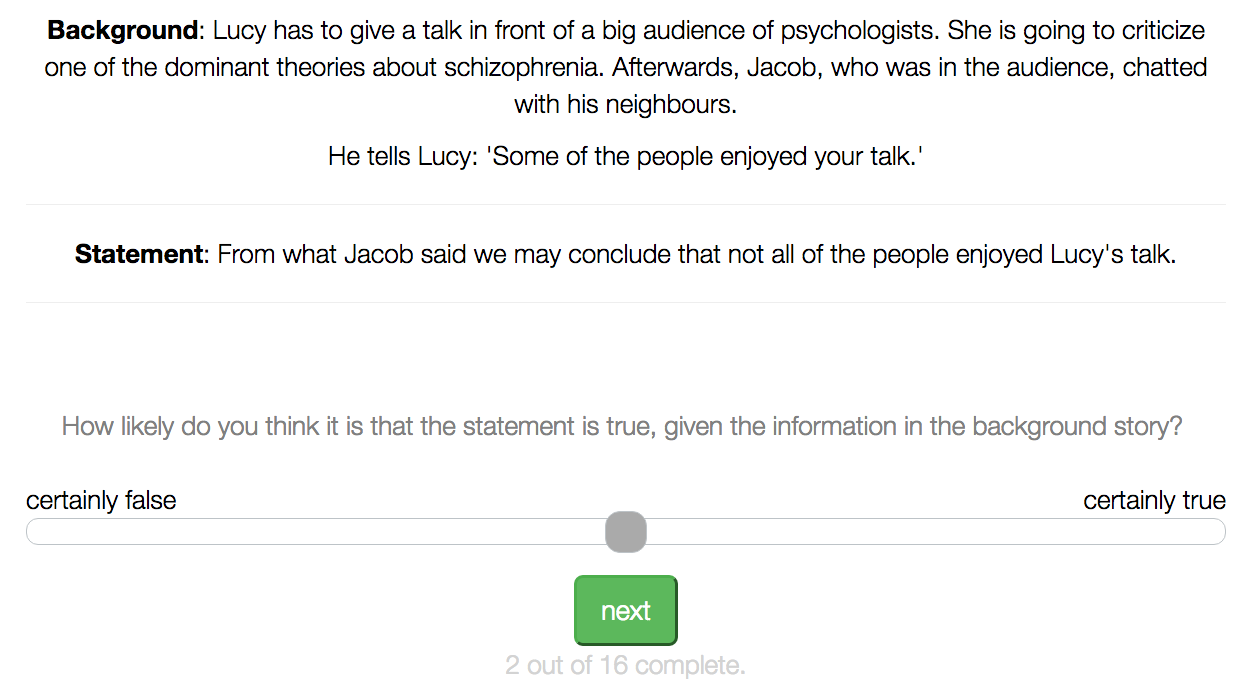
\includegraphics[width = 0.8\textwidth]{pics_02/expExampleShot_Lucy.png}
  \caption{Example of a trial from Exp.~1}
  \label{fig:exampleShot}
\end{figure}

%--------------------------------------------------------
\subsection*{Data preparation} 
%--------------------------------------------------------

We coded the slider-ratings as real numbers ranging from 0
(``certainly false'') to 1 (``certainly true''). Ratings for the two conditional statements in the prior condition of Exp.\ 2 were averaged.

Four participants were excluded from the analyses of Exp.~1 because they were not self-reported
native speakers of English; three for Exp.~2. We also removed another six (Exp.~1) and five
(Exp.~2) participants for obviously deviant answers (e.g., blindly alternating between maximal
agreement and maximal disagreement).\footnote{The formal criterion for exclusion was having a
  \emph{deviance score} greater than a fixed threshold, where the deviance score of a
  participant is the sum of the absolute differences between the expected answers for all
  control questions (0, 0.5, or 1) and the subjects'
  answers. % The mean deviance score was 1.758; its standard deviation is 0.862.
  We set the threshold of exclusion to the mean plus twice the standard deviation of all
  deviance scores. This exclusion criterion was also used in all other experiments.}
Consequently, data from a total of 193 (Exp.\ 1) and 192 (Exp.\ 2) participants made it into
our analysis. Unfortunately, there was a mistake in the formulation of two stories, one for
each experiment. We removed all data for these stories for the analysis. (See
Appendix~\ref{sec:mater-exper-1} and~\ref{sec:mater-exper-2}, especially
footnotes~\ref{fn:NBA_exp1} and~\ref{fn:order_exp2}.)

%--------------------------------------------------------
\subsection*{Results}
%--------------------------------------------------------

\paragraph{Controls.} Control statements were rated as expected, indicating that participants
understood the task and paid attention to the background stories. For Exp.~1, the averages over
all stories of ratings for false (0.21), uncertain (0.40) and true statements (0.80) are
pairwise different (two-population directed Welch's $t$-test: $t \approx - 4.04$,
$df \approx 27.9$, $p < 0.001$ for false vs.~uncertain; $t \approx - 9.23$, $df \approx 27.8$
$p < 0.001$ for uncertain vs.~true). Similarly, for Exp.~2, the averages over all stories of
ratings for false (0.26), uncertain (0.48) and true statements (0.81) are pairwise different
(two-population directed $t$-test: $t \approx - 3.92$, $df \approx 26.6$, $p < 0.001$ for false
vs.~uncertain; $t \approx - 7.20$, $df \approx 27.1$, $p < 0.001$ for uncertain vs.~true).

\paragraph{Explanatory factors.} We are interested in whether the ratings of statements for
relevance, competence and prior probability are good explanatory factors of the strength of
the upper-bounded construal of ``some'' (Exp.~1) or of the strength of the exclusive readings of ``or'' (Exp.~2). We
therefore look at explanatory factors \rel, \com and \pri, which are the means of the ratings,
for each story, of the \emph{Relevance}, \emph{Competence} and \emph{Prior} statements. Before
turning to our main analysis, we begin with a few observations about these explanatory factors.

First of all, ratings of the relevant statements are not uniformly
distributed across stories, but validate our intuitive pre-classification (see
Figure~\ref{fig:EFbars12}, all high/low contrasts are significant).
%
\begin{figure}
  \centering

  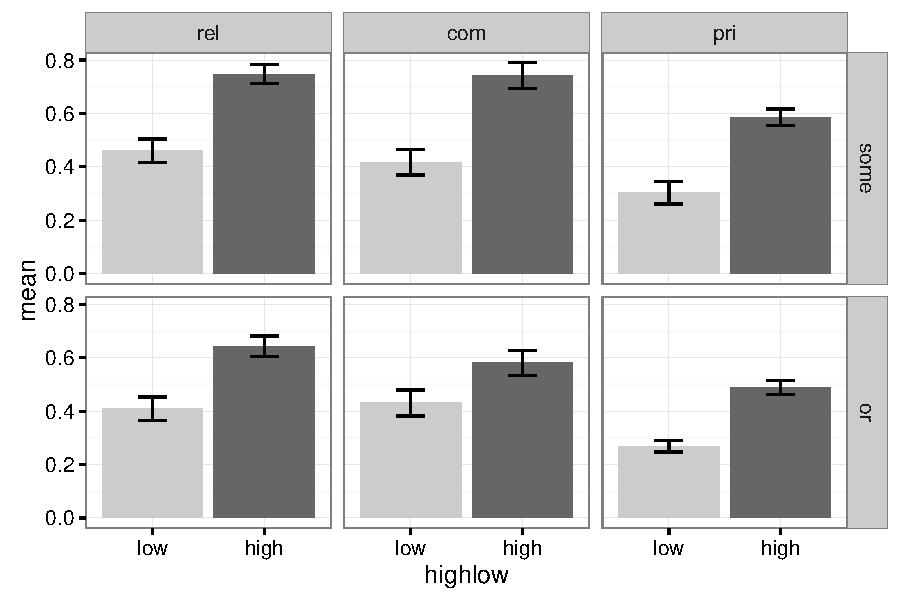
\includegraphics[width = 0.9\textwidth]{pics_02/EFbarsExp12.pdf}
  
  \caption{Ratings of statements according to intuitive pre-classification. Results for
    Exp.~1 (``some'') in the top row, results for Exp.~2 (``or'') in the bottom
    row. Error bars indicate bootstrapped 95\% confidence intervals around the plotted means.}
  \label{fig:EFbars12}
\end{figure}
%
Moreover, Figure~\ref{fig:correlationsExp12} shows how \rel, \com and \pri correlate with the
mean ratings of the strength of the upper-bounded construal of ``some'' and of the strength of the exclusive readings of
``or''. From visual inspection, it seems that in Exp.~1 (``some'') \rel and \com are not
likely to be strong predictors of the strength of the upper-bounded reading, while low values of \pri seem to be
correlated with high ratings, as expected. For Exp.~2 (``or''), the plots suggest
that \rel might not be correlated with the reported strength of exclusive readings, while there
do seem to be noteworthy correlations with \com and \pri. Interestingly if
exclusive readings of ``or'' are like bona-fide scalar implicatures, we should expect
higher values of \com to be associated with higher endorsements of exclusive
readings. What we observe, however, appears to be the opposite relation.

\begin{figure}
  \centering

  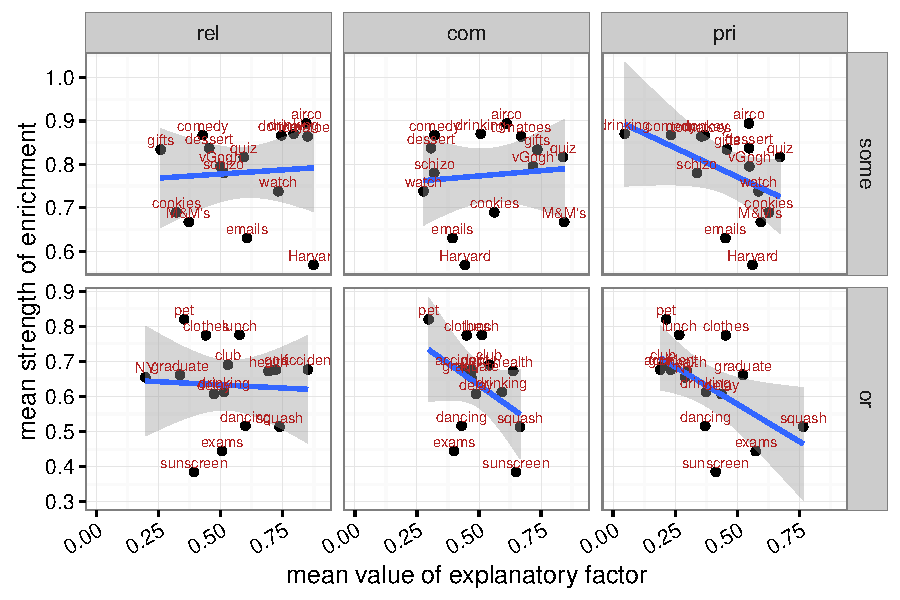
\includegraphics[width = \textwidth]{pics_02/correlationExp12.pdf}
  
  \caption{Relating ratings for relevance, competence and prior statements ($x$-axis) to
    ratings for the strength of pragmatic enrichments ($y$-axis). The top row shows ratings,
    averaged for each story, for Exp.~1 (``some''). The bottom row shows ratings,
    averaged for each story, for Exp.~2 (``or'').}
  \label{fig:correlationsExp12}
\end{figure}

In the light of subsequent regression models, it is important to note here that there is no
significant correlation between any pair of \rel, \com and \pri for neither experiment. That is,
the measures of \rel and \com for all stories of Exp.~1 are not correlated, neither are these
of \rel and \pri, et cetera.

\paragraph{Main analysis.} To check whether factors \rel, \com and \pri have an influence on
the ratings of the \emph{Inference}-statements---i.e., the strength of the upper-bounded construal in Exp.~1 and
of the exclusive reading in Exp.~2---we compare regression models of different
complexity. We take a Bayesian approach to model comparison here in terms of their Bayes
factors \citep{RouderMorey2012:Default-Bayes-F}, as implemented in the \emph{BayesFactor}
$R$-package. This gives us an intuitively accessible and quite nuanced picture of the relative
evidence for models of different complexity, including information about how much, e.g., the
absence of a factor in a model, is supported by our data.\footnote{All conclusions of
  theoretical relevance are also supported by more traditional, frequentist regression analyses
  in terms of significance of factors and model comparison by AICs.}

\begin{figure}
    \centering
    \begin{subfigure}[b]{0.49\textwidth}
      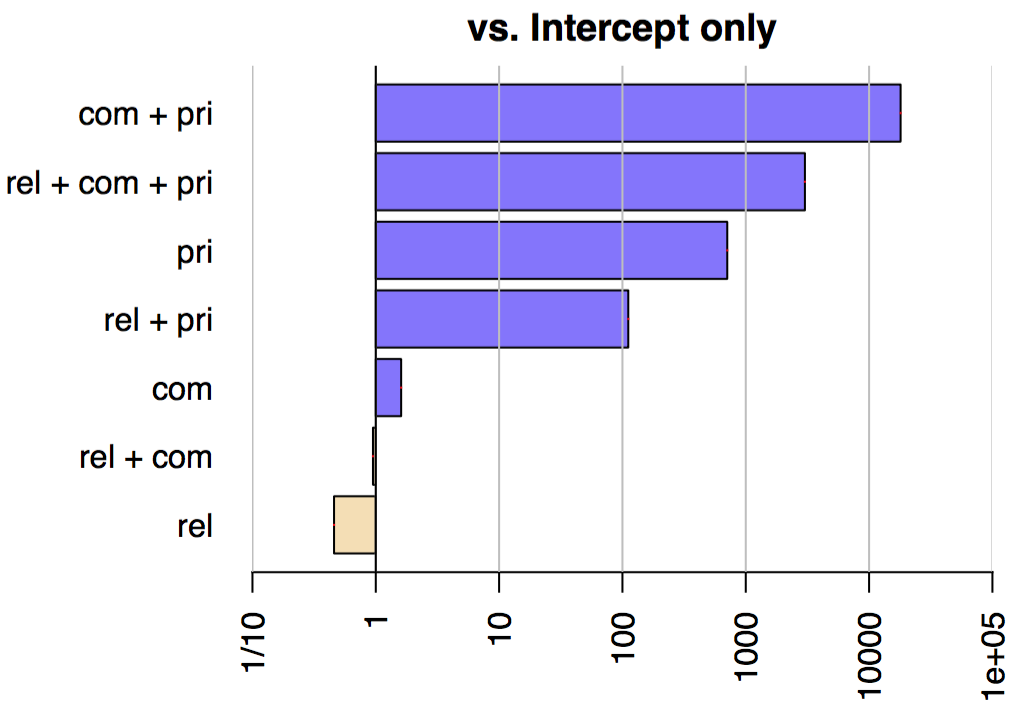
\includegraphics[width = \linewidth]{pics_02/bfsAllExp1_cropped.png}
  \caption{Exp.~1 (``some'')}
  \label{fig:BFsExp1}
    \end{subfigure}
    \hfill
    \begin{subfigure}[b]{0.49\textwidth}
      \centering
      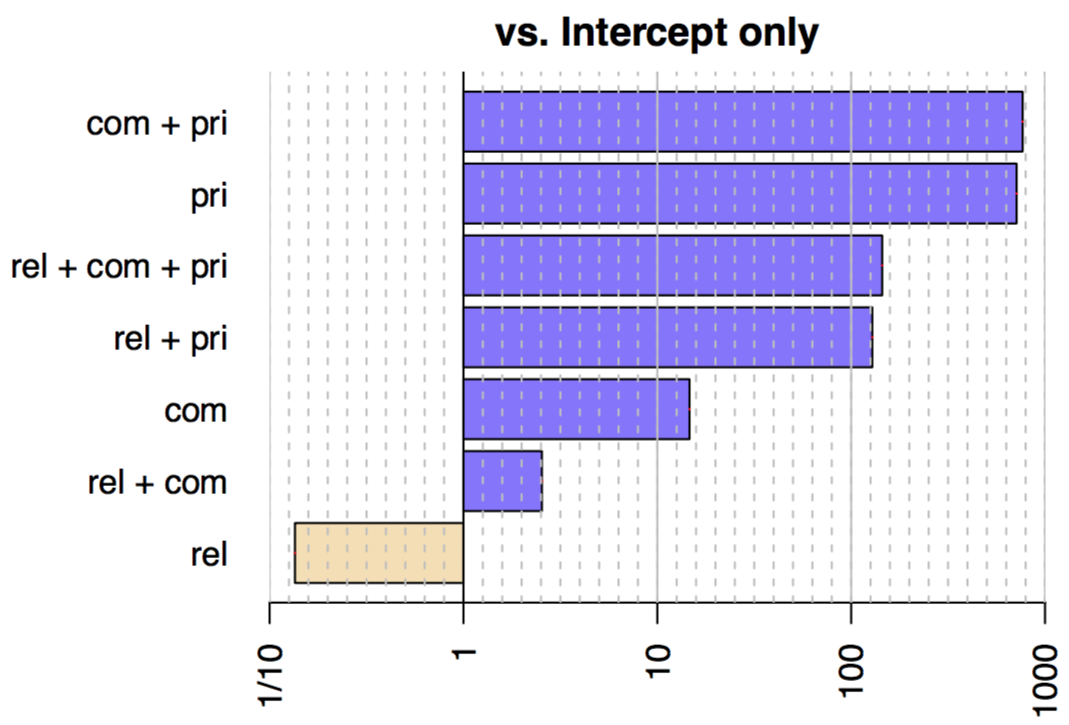
\includegraphics[width = \textwidth]{pics_02/bfsAllExp2_cropped.png}
      \caption{Exp.~2 (``or'')}
      \label{fig:BFsExp2}
    \end{subfigure}
    \caption{Bayes factor comparison of different main factor combinations. Notation like ``com
      + pri'' stands for a regression model with main factors \com and \pri. The plots show the
      Bayes factor on the logarithmic $x$-axis of the models on the left, when compared to an
      intercept only regression model.}\label{fig:BFs}
\end{figure}

Figure~\ref{fig:BFs} shows the Bayes factors of all regression models that can be built with
our three explanatory variables as main factors. The graphs give the Bayes factors of each
regression model listed on the left against the intercept-only model. Given the data from
Exp.~1, for example, the best model has main factors \com and \pri. It is more than 10,000
times more likely than the intercept only model. The model with the lowest a posteriori
likelihood is a regression model that contains only factor \rel, which is even worse than the
intercept-only model. Given the data from Exp.~2, the best and worst models are the same, but
there are differences as to how likely some of the other models appear to be, in the light of
the data.

For Exp.~1, the best model \com + \pri is very close to six times more likely than the full
model \rel + \com + \pri, which in turn, is about four times more likely than the model
\pri. It is common to consider Bayes factors above 3 as sufficiently noteworthy evidence in
favour of a model
\citep[e.g.][]{Jeffreys1961:Theory-of-Proba,Raftery1995:Bayesian-Model-,LodewyckxKim2011:A-tutorial-on-B}. The
picture that emerges is that, for Exp.~1, the addition of factors \pri and \com increases the a
posteriori likelihood, while the addition of factor \rel actually decreases it. This suggests
that the former are explanatory factors whose inclusion may make a model more complex but also
leads to better predictions. In contrast, the added model complexity of including \rel is not
countered by a similar increase in predictive power; we are better off without factor \rel.

Turning to Exp.~2, the best model \com + \pri is not noteworthily better, in terms of Bayes
factors, than the second best model which only includes \pri. Still, both of these models come
up noteworthily more likely, given the data, than the third best model, the full model with
\rel + \com + \pri: a Bayes factor of around five. The overal picture that emerges in this case
is that adding \rel to a model seems to decrease a posteriori likelihood, while adding
\com or \pri increases it. The most important single factor clearly is \pri: when a model
contains \pri, adding \com does not lead to substantial improvements. The main conclusion to be
drawn from this analysis is that \rel is a bad, \com an unnecessary, and \pri the best
predictor of strength of exclusive readings.\footnote{This general conclusion is also
  vindicated by more complex analyses that would take interactions and random effects for
  participants into account.}

Finally, inspired by previous observations based on Figure~\ref{fig:correlationsExp12}, let us
also look at the way that speaker competence influences the \emph{Inference}-ratings in each
experiment. What can be gleaned already from the plots in Figure~\ref{fig:correlationsExp12},
is supported by inspection of estimates of regression
coefficients. Figure~\ref{fig:densityMCMC} shows posterior distributions for regression
coefficients of the full model \rel + \com + \pri after conditioning with the data from Exp.~1
(top row) and Exp.~2 (bottom row). We see that credible values for coefficients for \com are
positive for Exp.~1, as expected, but mostly negative for Exp.~2. This means that our data
suggest that the more competent the speaker was felt to be, the lower the strength of the
exclusive reading. This is the inverse of what a scalar implicature account would suggest and
also the inverse of what we find for the upper-bounded construal of ``some''. 

\begin{figure}
  \centering
  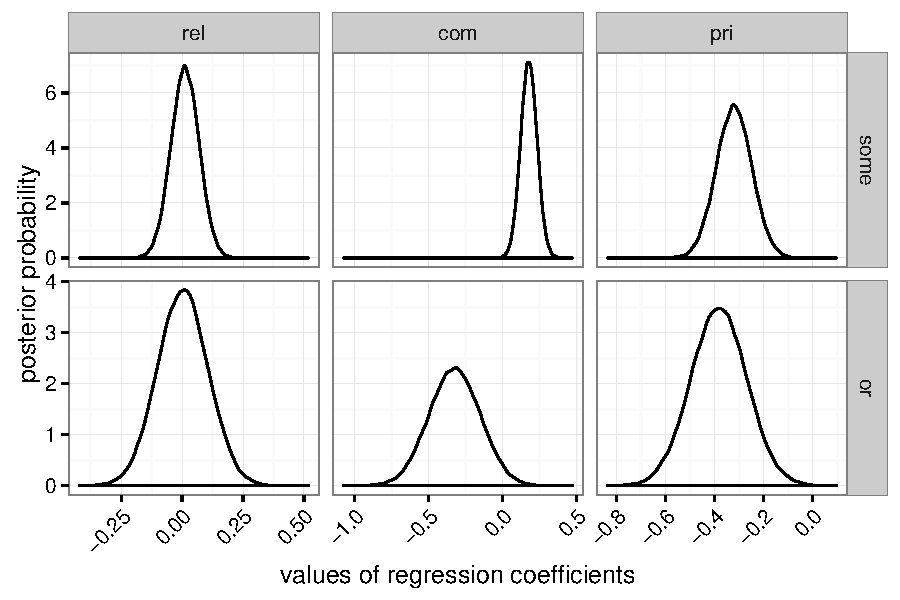
\includegraphics[width=0.8\textwidth]{pics_02/densityMCMCExp12.pdf}
  \caption{Density estimates of posterior over model parameter coefficients for a linear model
    with all three main factors.}
  \label{fig:densityMCMC}
\end{figure}

\paragraph{Discussion.} The main explanatory factors for \emph{Inference}-ratings for ``some''
appear to be the speaker's competence and the prior probability of the ``all''-alternative. These
findings are not unexpected under standard scalar implicature accounts except, perhaps, that
there does not seem to be the predicted influence of relevance. As for ``or'', it seems that
prior probability of the stronger alternative is the main explanatory factor of
\emph{Inference}-ratings. In contrast to the results for ``some'', there does not seem to be a
strong effect of speaker competence on the perceived strength of exclusive readings. This is
surprising under standard scalar implicature theories of exclusive ``or'', even more so when we
also consider the ``direction'' of the relation between speaker competence and inference
ratings. While in Exp.~1 higher speaker competence correlated with higher scalar implicature
inference rates, this relationship was reversed in Exp.~2, contrary to the expectations
generated by a standard scalar implicature account of exclusive inferences.

These findings thus appear to jeopardise the standard scalar implicature account of exclusive
disjunction. Before drawing firm conclusions, however, the next section first considers an
alternative approach that is similar to the standard account in that it assumes that the
exclusive reading of ``or'' is a conversational implicature, but that is also different from
the standard account in a number of important respects.



%---------------------------------------
\section{Experiment~3}
%---------------------------------------

\subsection*{Motivation}

There is a much less prominent alternative approach to deriving exclusive disjunction readings
as a conversational implicature. We will refer to it as the \emph{distinct disjuncts} account
here. It takes as its point of departure the observation that statements with ``or'' tend to be
infelicitous when there is some overlap between the propositions that the individual disjuncts
express \citep{hurford1974, simons2001, ZimmermannFreeChoiceDisjunction2000}. Hence, the
following sentences appear to be pragmatically marked:

\ex.	\a. \label{ex:hurford} Ivan is an American or a Californian.
	\b. That painting is of a man or a bachelor.
	
The reason for this infelicity is that being a Californian entails being an American, and that being a bachelor entails being a man. Hence, there is overlap between the disjuncts, which violates the distinctness condition.

In addition, statements with ``or'' are infelicitous unless both disjuncts are answers to some question under discussion \citep{simons2001}. For that reason, B's answer in the following exchange is infelicitous:

\ex.	A: Where is Donald? \\ B: He is in his room or fleas are annoying.

The reason for this infelicity is that it is difficult to imagine that the information that fleas are annoying provides an adequate answer to the question that A asked. Since one of the disjuncts fails to provide an adequate answer to the question under discussion, the entire statement comes out as infelicitous.

A final relevant observation is that answers to questions tend to be interpreted exhaustively. To illustrate, consider the following dialogue:

\ex.	A: Who does Joe support? \\ B: Donald.

Here, B's answer will be construed as implying that Joe supports Donald but not Hillary. In other words, B's answer is interpreted as being exhaustive. Exhaustivity in answers is usually explained as a conversational implicature along the following lines:\ if B knew that Joe supports, e.g., both Donald and Hillary, it would have been informative and relevant to mention that. Since he did not, the hearer may conclude that, according to B, Joe supports Donald but not Hillary.

Given that disjuncts have to provide an answer to the question under discussion, and given that answers to questions tend to be interpreted exhaustively, one might propose that disjuncts are interpreted exhaustively, too \citep{fox2007,ZimmermannFreeChoiceDisjunction2000}. According to this proposal, a statement of the form ``$A$ or $B$'' may be read, in effect, as ``$A$ but not $B$ or $B$ but not $A$''. To illustrate, consider \ref{ex:support} once again:

\ex.	Joe supports Donald or Hillary.

According to the distinct disjuncts account, an utterance of this sentence may be interpreted, in effect, as ``Joe supports Donald but not Hillary or Hillary but not Donald.'' This interpretation is exclusive, since the disjuncts cannot both be true.

% The distinct disjuncts account explains the aforementioned distinctness condition:\ \ref{ex:hurford} is infelicitous because it is read as ``Ivan is an American but not a Californian or a Californian but not an American''. Since the latter disjunct is a contradiction, the entire statement comes out as infelicitous. In a sense, then, the present proposal forces the disjuncts to be distinct.

If the distinct disjuncts account is on the right track, we should expect that the robustness of the exclusive reading increases with the robustness of the exhaustive reading associated with an utterance of one of the disjuncts. In other words, the robustness of the exclusive reading of \Last should increase with the robustness of the inference from ``Joe supports Donald'' to ``Joe supports Donald but not Hillary'' and with the robustness of the inference from ``Joe supports Hillary'' to ``Joe supports Hillary but not Donald''.

\subsection*{Design}

The distinct disjuncts account predicts that the strength of an exclusive reading of ``$A$ or $B$'' should be positively correlated with the strength of exhaustive readings that statements of individual disjuncts $A$ and $B$ would receive in the same context. The purpose of Exp.~3 was therefore to collect data on the strength of
exhaustive readings of such single-disjunct statements in the background contexts used in
Exp.~1. We would then like to investigate whether strengths of exhaustive readings are a
reliable predictor of strength of exclusive readings across contexts.

\subsection*{Participants}

Using the same selection criteria as before, 131 subjects were recruited via Amazon's
Mechanical Turk and paid US\$ 0.50 for participation.

\subsection*{Materials}

Exp.~3 used the fifteen stories that entered the analysis of Exp.~2. For each story we consider
the speaker's utterances of single disjuncts. Concretely, where Exp.~2 had an utterance of a
sentence:

\begin{center}
\begin{tabular}{p{10cm}}
  \emph{Utterance of disjunction}\\
  Jill says to Danny: ``Alex bought a racket or a pair of shoes.''
\end{tabular}
\end{center}

\noindent Exp.~3 had two single-disjunct utterances by the same speaker:

\begin{center}
\begin{tabular}{p{10cm}}
  \emph{Utterance of disjunct 1}\\
  Jill says to Danny: ``Alex bought a racket.'' \\[.2cm]
  \emph{Utterance of disjunct 2}\\
  Jill says to Danny: ``Alex bought a pair of shoes.''
\end{tabular}
\end{center}

\noindent Each story also had corresponding statements that subjects had to
rate:

\begin{center}
\begin{tabular}{p{10cm}}
  \emph{Exh1}\\
  From what Alex's girlfriend said we may conclude that Alex did not buy a pair of shoes as well. \\[.2cm]
  \emph{Exh2}\\
  From what Alex's girlfriend said we may conclude that Alex did not buy a racket as well.
\end{tabular}
\end{center}

\subsection*{Procedure}

The procedure followed that of Exp.~2 very closely. After reading the slightly amended
instructions and seeing examples for the use of the slider bar, each participant was presented
with six randomly sampled stories. Subjects read the background story, followed by an
utterance of either disjunct, randomly chosen. Subjects first rated a random control question
and then rated the \emph{Exh1} or \emph{Exh2} statement, depending on which utterance was shown
to them.

\subsection*{Results}

Data from one subject was discarded because English was not the self-reported native
language. Another four subjects were removed for bad performance on the control questions,
using the same criterion as before.

\begin{figure}
  \centering
  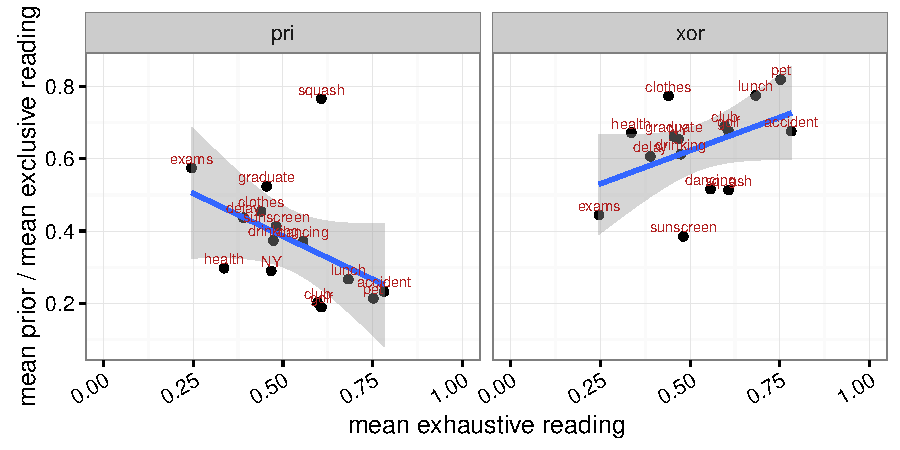
\includegraphics[width=0.9\textwidth]{pics_02/correlationExhXorPri.pdf}
  \caption{Means of ratings of \emph{Exh}-statements from Exp.~3 ($x$-axis) vs. means of
    ratings of \emph{Prior}-statements and \emph{Xor}-statements from
    Exp.~2 ($y$-axis)}
\label{fig:CorrelationExp1Exp4}
\end{figure}

Figure~\ref{fig:CorrelationExp1Exp4} shows the per-story means of the ratings of the
\emph{Exh}-statements plotted against the corresponding mean ratings of the \emph{Prior}- and
\emph{Xor}-statements from Exp.~1. There is no significant correlation between
\emph{Prior}-ratings and \emph{Exh}-ratings ($r \approx -0.45$, $p \approx 0.09$), suggesting
that our measures of prior expectations and exhaustive strength do not coincide. Adding the
per-story mean \emph{Exh}-ratings as an additional explanatory factor \exh to the regression
model comparison, we obtain the picture given in Figure~\ref{fig:BayesFactorsExp4}. A model
using single factor \pri to predict \emph{Xor}-ratings is about 8.5 times more likely than a
model using single factor \exh. That means that our data provides evidence for the assumption
that prior expectations are a better explanatory factor of exclusive readings than the strength
of exhaustive readings, thus discounting the distinct disjuncts account.

\begin{figure}
  \centering
  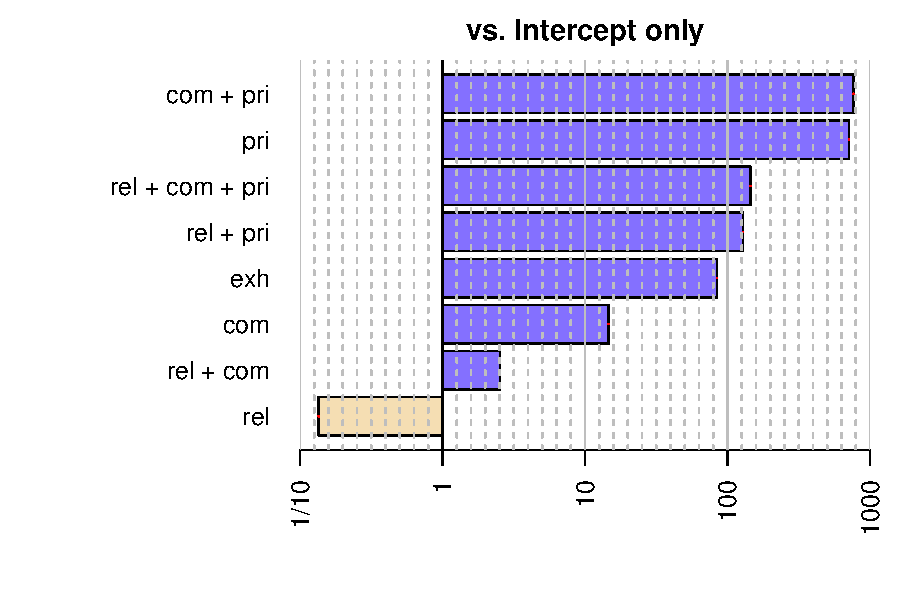
\includegraphics[width=0.9\textwidth]{pics/bfsAllExp4.pdf}
  \caption{Bayes factor comparison of different main factor combinations, predicting the
    strength of exclusive disjunction readings with additional factor \exh from Exp.~3.}
\label{fig:BayesFactorsExp4}
\end{figure}

%------------------------------------------
\section{General discussion}
%------------------------------------------

Statements of the form ``$A$ or $B$'' are sometimes interpreted as ``$A$ or $B$ but not both''. The
consensus in the recent literature is that these exclusive readings are scalar implicatures,
which are inferences deriving from a pragmatic reasoning process about the speaker's
intentions. A crucial assumption in this reasoning process is that the speaker is taken to be
knowledgeable about whether the corresponding statement with ``$A$ and $B$'' is true. In this
paper, we have presented data that challenge the implicature account. In contrast to the
predictions made by this account, the robustness of the exclusive reading does not increase
with the competence of the speaker about ``$A$ and $B$''. Instead, we observed the reverse
effect.

We also tested an alternative proposal, according to which the exclusive reading is derived as
a conversational implicature by exhaustifying the individual disjuncts. According to this proposal, a
sentence of the form ``$A$ or $B$'' is read, in effect, as ``$A$ but not $B$ or $B$ but not $A$''. This proposal predicts that the robustness of the exclusive reading depends on
the robustness of the inference from $A$ to ``$A$ but not $B$''. Although we did find a
significant effect of this factor, it was a significantly worse predictor of the robustness of
the exclusive reading than the ratings of prior probability of the ``and''-alternative.

\paragraph{Exclusive readings and probabilistic world knowledge.} Taken together, these
findings suggest that the exclusive reading of ``or'' might not be a scalar
implicature. Instead, we propose that exclusive readings could be the result of probabilistic
inferences about the state of the world. In other words, the meaning of ``or'' is inclusive,
but hearers may exclude the possibility that both disjuncts are true based on their knowledge
of the world.

Such probabilistic inferences have been shown to influence various other parts of language. A case in point is quantifying expressions. In a series of experiments, Moxey and Sanford \citeyearpar{moxey1993} presented participants with statements such as:

\ex.	\a. $Q$ people found Miss Sweden attractive.
	\b. $Q$ earthquakes occurred in California in 1951.
	
$Q$ was varied between ten quantifying expressions, including ``a few'' and
``many''. Participants were instructed to estimate, e.g., the number of people who found Miss
Sweden attractive and the number of earthquakes in California in 1951, based on the information
expressed in the sentences. For most quantifying expressions, Moxey and Sanford observed that
these estimates increased as a function of the prior probability. For example, the estimates
would be higher for \Last[a] than \Last[b], since the prior probability that at most $n$ people
find Miss Sweden attractive is lower than the prior probability that at most $n$ earthquakes
occurred in California in 1951 (see also \citealt{pepper1974}). 

In a similar vein, the interpretation of vague gradable adjectives, such as ``big'' and
``small'', varies depending on our world knowledge. Kamp and Partee \citeyearpar{kamp1995}
discuss the following minimal pair:

\ex.	\a. My two-year old son built a really tall snowman yesterday.
	\b. The D.U. fraternity brothers built a really tall snowman yesterday.
	
It is obvious that one's prior expectations about the size of the snowman are lower in the case
of \Last[a] than in the case of \Last[b], thus demonstrating that the interpretation of ``tall''
varies depending on one's prior expectations. Recent probabilistic models of pragmatic language
use have explored this systematic dependence on prior expectations
\citep[cf.,][]{LassiterGoodman2015:Adjectival-vagu,QingFranke2014:Gradable-Adject,SchollerFranke2015:Semantic-values}.

World knowledge and prior expectations thus influence the interpretation of various aspects of
natural language. We propose that the interpretation of ``or'' is one such aspect as well:\
although, strictly speaking, a statement of the form ``$A$ or $B$'' leaves open the possibility
that both $A$ and $B$ are true, prior expectations can modulate the likelihood of this
possibility. If our proposal is on the right track, this would have important theoretical
repercussions. For instance, exclusive readings of sentences with ``or'' have been argued to occur in
embedded positions as well, i.e., in the scope of other logical operators, as in \Next, where
standard accounts might not (easily) predict scalar implicatures to arise. If exclusive
readings of disjunctions are no (ordinary) scalar implicatures, arguments based on their
occurrence in embedded position provide little motivation for a radical conceptual rethinking of
scalar implicatures \emph{tout court} \citep[e.g.,][]{chierchia2004,chierchia2012,fox2007}.

\ex. If you order pizza or pasta before 7pm, you pay only \$6.50.

\paragraph{Competence.} We compared ``or'' with ``some'', which is often interpreted as ``some but
not all''. This upper-bounded construal is an uncontroversial example of a scalar
implicature. Unlike the exclusive reading of ``or'', the robustness of the upper-bounded
construal of ``some'' increased with the competence of the speaker about the truth of the
corresponding statement with ``and'', in line with the results of Goodman and Stuhlm\"{u}ller
\citeyearpar{goodman2013}. 

It remains an open question for further research as to why higher ratings of speaker competence
seem to pair with lower prominence of exclusive readings. A possible line of explanation could
be to dissect the relationship between world states and speaker knowledge, and experimental
participants' intuitive model thereof. It is possible to imagine that world states where ``$A$
and $B$'' is false are more likely than states where this is not so to give rise to epistemic
states in which the speaker would use the statement with ``or'' and is ignorant about the
``all''-alternative. This could be because of asymmetries between observability of positive and
negative facts---it is usually easier to notice that Alex bought a racket than that he did
not---or because it may require more than simple observation for an agent to form a belief that
``$A$ or $B$, but not both'' or that ``$A$ iff $B$''. An integrated probabilistic model that
incorporates reasoning about evidence and language use, similar to that of Goodman and
Stuhlm\"{u}ller \citeyearpar{goodman2013}, which jointly infers a world state and an epistemic
state based on a speaker's utterance, might shed light on the puzzling relation between
competence and strength of exclusive readings that we observed. Since, presently, we can at
best conceive of entirely ad hoc models of how world states and epistemic states could be
related to each other, we must leave this issue for future research.

\paragraph{Prior probability.} We observed a significant effect of prior probability:\ the
robustness of the upper-bounded construal decreased with the prior probability that the
statement with ``all'' was true. This effect ties in with recent experimental work from
\citet{degen2015}, but speaks against observations made by \citet{geurts2010}. Geurts discusses
examples such as the following to show that the decision to derive a scalar implicature is made
independently from the prior probability that the statement with ``all'' is true.

\ex.	Cleo threw all her marbles in the swimming pool. Some of them sank to the bottom.

Here, according to Geurts' intuitions, the speaker communicates that some but not all of the
marbles sank to the bottom, even though such a situation has an extremely low prior
probability. It remains to be seen whether a probabilistic model along the lines of
\citet{degen2015} can account for the effects of priors and speaker competence that we observed
here, as well as for exclusive readings of ``or''.

\paragraph{Relevance.} Unlike competence and prior probability, relevance to the hearer's
interest did not turn out to have any effect on the robustness of the upper-bounded construal
of ``some''. This is problematic to relevance theory, which predicts the robustness of an
upper-bounded construal to be an increasing function of its importance to the hearer. It may
suggest that relevance theory should adopt a more restricted notion of relevance in terms of
discourse purposes \citep{cummins2015}. Alternatively, we might hold that hearer-oriented
relevance is only one specific case of discourse relevance. Accordingly, the absence of an
affect of relevance manipulations in our experiment may be a result of indeterminacy as to
which aspect of discourse relevance prevails. Still, if this were so, then our results would at
least indicate that hearer-oriented relevance is not a strong and dominant default.

An alternative explanation for the absence of an effect of relevance, however, is that
we did not manipulate how relevant the upper-bounded construal was to the
participant. According to this explanation, we failed to observe a significant effect because
there were no differences in how relevant the upper-bounded readings were to the
participants. Even though this alternative explanation warrants closer examination, there are
several reasons to be skeptical about it. Perhaps the most prominent reason is that, strictly
speaking, participants did not have any reason to derive the scalar implicature in the first
place. The fact that they did so nonetheless indicates, from a relevance-theoretic point of view,
that they engaged with the story.

In summary, then, our results provide an insight in how various factors conspire in shaping
differences in the robustness of putative scalar implicatures. It will be interesting to
determine which other factors---e.g., typicality \citep{tiel2013}, prosodic and linguistic
prominence \citep{breheny2006}, and politeness \citep{bonnefon2009}---have similar effects, and
how these factors might interact. It may well be that these factors also hold the key to
explaining the observation that different scalar expressions license scalar implicatures at
substantially different rates \citep{tiel2016}. Such questions, however, remain for the moment
as topics for future research.

\bibliography{bibliography}

%--------------------------------------------------------------
\appendix
%--------------------------------------------------------------

%--------------------------------------------------------------
\section{Stories from Experiment 1}
\label{sec:mater-exper-1}
\input{stories_exp1.txt}
%--------------------------------------------------------------

%--------------------------------------------------------------
\section{Stories from Experiment 2}
\label{sec:mater-exper-2}
\input{stories_exp2.txt}
%--------------------------------------------------------------

\normalsize

\newpage

\listoffigures

\newpage 

\theendnotes

\end{document}
